\documentclass[conference]{IEEEtran}
\IEEEoverridecommandlockouts

% Language setting
% Replace `english' with e.g.
\usepackage[english]{babel}


% Useful packages
\usepackage{amsmath}
\usepackage{graphicx}
\usepackage{csquotes}
\usepackage[colorlinks=true, allcolors=blue]{hyperref}
\usepackage[shortlabels]{enumitem}
\usepackage{textcomp}
\usepackage{cleveref}

% Bibliography
\usepackage[
    backend=biber,
    style=ieee,
    natbib,
    mincitenames=1,
    maxcitenames=1,
    uniquelist,
    doi=false,
    url=false,
    sorting=none,
    maxbibnames=10,
]{biblatex}
\addbibresource{sample.bib}
%\addbibresource{bib-leo.bib}

% Acronyms
\usepackage[acronyms]{glossaries}
\newacronym{fl}{FL}{Federated Learning}
\newacronym{ml}{ML}{Machine Learning}
\newacronym{dl}{DL}{Deep Learning}
\newacronym{ids}{IDS}{Intrusion Detection System}
\newacronym{fids}{FIDS}{Federated Intrusion Detection System}
\newacronym{cids}{CIDS}{Collaborative Intrusion Detection System}
\newacronym{ai}{AI}{Artificial Intelligence}
\newacronym{siem}{SIEM}{Security Information and Event Management}
\newacronym{niid}{NIID}{Non Identically or Independently Distributed}
\newacronym{cdfl}{CD-FL}{Cross-Device Federated Learning}
\newacronym{csfl}{CS-FL}{Cross-Silo Federated Learning}

\glsdisablehyper

% Abbreviations
\usepackage{xspace}
\makeatletter
\DeclareRobustCommand\onedot{\futurelet\@let@token\@onedot}
\def\@onedot{\ifx\@topicslet@token.\else.\null\fi\xspace}
\def\eg{\emph{e.g}\onedot} \def\Eg{\emph{E.g}\onedot}
\def\ie{\emph{i.e}\onedot} \def\Ie{\emph{I.e}\onedot}
\def\cf{\emph{cf}\onedot} \def\Cf{\emph{C.f}\onedot}
\def\etc{\emph{etc}\onedot} \def\vs{\emph{vs}\onedot}
\def\wrt{w.r.t\onedot} \def\dof{d.o.f\onedot}
\def\etal{\emph{et al}\onedot}
\makeatother

\usepackage{titlesec}
% \titleformat{\paragraph}% command
% [runin]% shape
% {\normalfont\bfseries}% format
% {\alph{paragraph}) }% label
% {0em}% sep
% {}% before-code
% [.]% after-code

% \titlespacing*{\paragraph}% command
% {0pt}% left
% {0pt}% before-sep
% {1em}% after-sep


\titleformat{name=\paragraph,numberless}% command
[runin]% shape
{\normalfont\itshape}% format
{}% label
{0em}% sep
{}% before-code
[:]% after-code
\titlespacing*{name=\paragraph,numberless}
{\parindent}% left
{0pt}% before-sep
{*1}% after-sep

\begin{document}

\title{Tutorial: Federated Learning $\times$ Security\\ for Network Monitoring}
\author{
\IEEEauthorblockN{Yann Busnel}
\IEEEauthorblockA{\textit{Institut Mines-Télécom} \\ % dept.
name of organization (of Aff.)
Palaiseau, France \\ % City, Country
\url{yann.busnel@imt.fr}} %email address or ORCID
\and
\IEEEauthorblockN{Léo Lavaur}
\IEEEauthorblockA{\textit{SnT, University of Luxembourg} \\ % dept.
name of organization (of Aff.)
Luxembourg \\ % City, Country
\url{leo.lavaur@uni.lu}} %email address or ORCID
}

\maketitle

\begin{abstract}
    \Gls{fl} is a distributed learning paradigm that enables training models across distributed clients without accessing their data.
    In the context of network security, \gls{fl} can be used to collaboratively train \gls{ids} models across multiple organizations, allowing participants to share knowledge without compromising data privacy.
    However, the distributed nature of \gls{fl} raises new challenges, notably the heterogeneity of clients' data distributions and the identification of malicious contributions.
    
    This three-part tutorial introduces the audience to (i) the principles of \gls{fl}, (ii) its application to network security, focusing on building \glspl{cids} using \gls{fl}, and (iii) the security challenges associated with deploying \gls{fids}, with a focus on poisoning attacks.
    Each part is illustrated with hands-on exercises, with step-by-step instructions provided in the companion material.
\end{abstract}

\glsresetall

\begin{IEEEkeywords}
Federated Learning, Network Security, Collaborative Intrusion Detection System, Network Monitoring, Data poisoning.
\end{IEEEkeywords}

\section{Introduction} % Yann

\gls{fl} has emerged as a promising paradigm for collaborative machine learning, enabling model training across decentralized data sources without compromising privacy.
It quickly became prevalent in the distributed systems' community, with applications ranging from healthcare to fraud detection.
In the context of network security, \gls{fl} offers a compelling solution to the challenges of training \gls{ids} models across multiple organizations, allowing participants to share knowledge without compromising data privacy.
Yet, this use case comes with its own set of challenges, notably due to the heterogeneity of clients' data distributions.

\subsection{Motivation}

This tutorial delves into the fundamentals of \gls{fl}, exploring its core principles and applications (\Cref{sec:fl}), with a focus on collaborative network security.
The topic is particularly relevant for the distributed system community, as it echoes to a lot of the challenges faced in this field.
The aim is to establish a solid foundation for understanding the subsequent discussions on the applications of \gls{fl} in collaborative network security and the associated security challenges.
Previous iterations of this tutorial have been held at various venues, including the 14th IEEE/Comsoc International Conference on Networks of the Future (NoF) in October 2023~\cite{lavaur_nof_tuto_2023} and the 2024 IEEE International Conference on Distributed Computing Systems (ICDCS)~\cite{lavaur_icdcs_tuto_2024}.
However, due to organizational issues at the last ICDCS edition, the tutorials had underwhelming attendance, which limited the benefits of our interactive approach.
Despite this, we believe that the number of FL-related tracks and workshops planned at ICDCS 2025 highlights the increasing interest of this community for \gls{fl} and its applications, including distributed network security.

\subsection{Tutorial content}

The tutorial is divided into three parts, each doubled with hands-on exercises to provide participants with practical insights into the complexities of collaborative network security using \gls{fl}.
Specifically, the tutorial covers the following.
\begin{enumerate}[(i)]
    \item \emph{Fundamentals of Federated Learning} (\Cref{sec:fl}), where participants are introduced to the core principles of \gls{fl} and its applications.
    \item \emph{\gls{fl} for Collaborative Network Security} (\Cref{sec:fids}), focusing on the application of \gls{fl} to network security, and more specifically to the training of \gls{cids} models.
    \item \emph{Security Challenges in FL} (\Cref{sec:threats}), addressing the challenges of deploying and running \glspl{fids}, with a focus on poisoning attacks and mitigation strategies.
\end{enumerate}

\paragraph*{Hands-on}

Through examples and hands-on exercises provided in the companion repository\footnote{Available at: \url{https://github.com/leolavaur/icdcs_2025}}, the audience should gain insights into practical implementation of \gls{fl} using Flower~\cite{beutel_Flowerfriendlyfederated_2020}, an open-source Python framework.
Hands-on activities involve constructing a basic \gls{cids} model using Flower and experimenting with real-world network traffic datasets, providing participants with practical insights into tackling the complexities of collaborative network security using \gls{fl}.
Through interactive exercises, attendees can also simulate and analyze poisoning attacks on \gls{cids} models, along with devising and testing mitigation strategies to safeguard against such threats.

\subsection{Practical implementation}

\paragraph*{Target audience and prerequisites}

This tutorial is open to anyone (M.Sc.
to Faculty) with basic knowledge of machine learning (particularly neural networks) and Python programming.
A grasp of networking and cybersecurity concepts is a plus, but not required.
No prior knowledge of \gls{fl} is needed, as we will go over the core principles of \gls{fl} in the first part.

There is no technical limit to the number of participants, but the hands-on exercises will be more interactive with a smaller group (30--40 participants).
More participants can be accommodated, in which case the hands-on part will be more of a demonstration.

\paragraph*{Provided materials}
% Describe any materials the tutors intend to distribute, including size, media format, etc.
%Please note that the materials themselves need not be provided in the proposal

The tutorial will be supported by slides and Jupyter notebooks, which will be distributed to the participants before and after the tutorial, respectively.
The slides will be in PDF format and include references to the literature for further reading.
The Jupyter notebooks will contain step-by-step instructions and code snippets to fill, and installation instructions will be provided beforehand for the required dependencies (such as NumPy, Pandas, Matplotlib, TensorFlow, Flower\dots).
However, attendees must be warned that issues with their environment will not be addressed during the tutorial and that deep learning frameworks can be resource-intensive.
Alternatively, the Jupyter notebooks will also be loadable in Google Colab, so that participants can run them directly in their browser without any installation, albeit with potential limitations on the available resources.

\subsection{Paper content}

The rest of this paper summarizes the tutorial content, starting with the fundamentals on \gls{fl} in \Cref{sec:fl}, its application to network security in \Cref{sec:fids}, and the challenges associated with its security in \Cref{sec:threats}.
Additionally, biographies for the two speakers, Yann Busnel and Léo Lavaur, can be found at the end of this document.


\section{Fundamentals of Federated Learning\label{sec:fl}} % Yann
%% INTRODUCTION TO \gls{fl}

\Gls{fl} emerges at the intersection of collaborative computing and machine learning paradigms, offering a revolutionary approach to training models across a distributed network of devices without centralized data aggregation.
Rooted in the concept of crowdsourcing, where large groups contribute or produce goods and services, \gls{fl} extends this notion to machine learning, enabling diverse participants, from smartphones to IoT devices, to collaboratively improve model performance while preserving data privacy.

% The genesis of \gls{fl} can be traced back to crowdsourcing platforms like Waze, where users collectively contribute real-time traffic data, or collaborative journalism initiatives, illustrating the power of decentralized contributions.
% Industrializing crowdsourcing further, \gls{fl} finds applications in various domains, marking a shift towards harnessing collective intelligence for data-driven tasks.

In its foundation, \gls{fl} addresses the limitations of centralized machine learning by distributing the learning process across multiple nodes, each possessing local data and processing capabilities.
This distributed approach not only enhances scalability to handle large datasets, but also mitigates privacy concerns associated with sharing sensitive data.
Thus, the motivation for \gls{fl} includes performance improvement with more data, meaningful combination of models and local training at node scale (and not only prediction at the edge).
By allowing nodes to collaborate on model updates without sharing raw data, \gls{fl} ensures privacy compliance with regulations such as HIPAA and GDPR, crucial in sensitive domains like healthcare and advertising.


%% EXPLANATION OF THE CORE FUNCTIONNING + FIGURE ??
\subsection{FL in a Nutshell}

At its core, unlike traditional centralized learning approaches, \gls{fl} does not require raw data to be uploaded to a central server.
The latter transmits an initial model to the participating nodes, usually generated randomly (\cf, \Cref{fig:fl-phase1}).
Then, the model updates are computed locally on each device based on its data and then shared with a central server or aggregator (\cf, \Cref{fig:fl-phase2}).
These updates are aggregated to construct a global model, which is subsequently refined and redistributed to the participating devices.
This iterative process continues, with each round of communication and aggregation improving the global model's accuracy without compromising the privacy of individual data.



\begin{figure}[t]
    \centering
    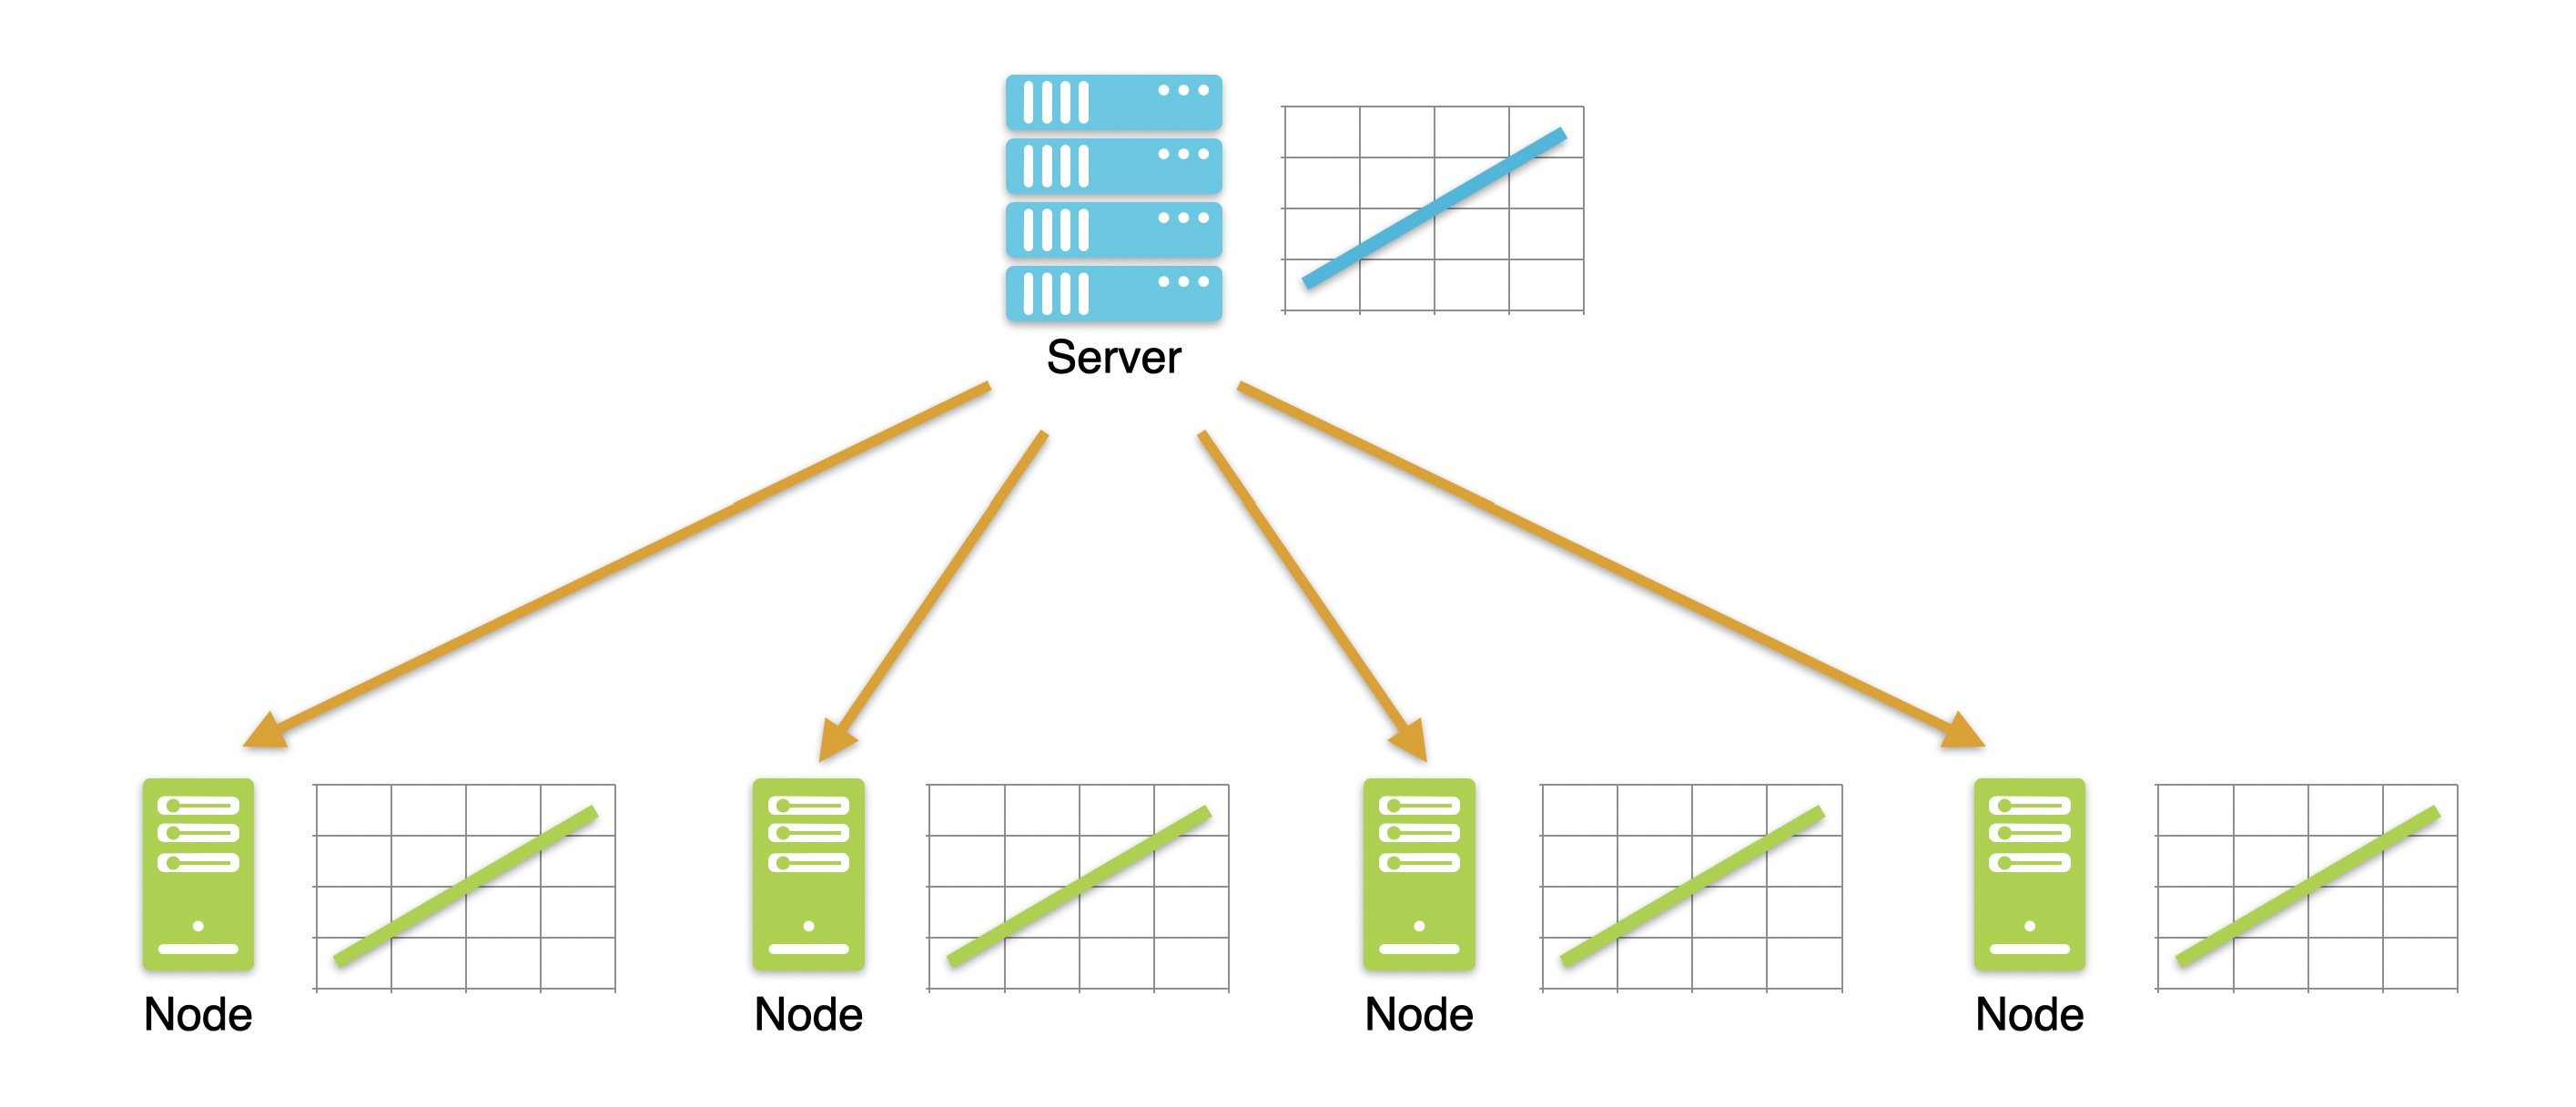
\includegraphics[width=\linewidth]{img/FL-phase1.jpg}
    \vspace*{-.8cm}
    \caption{First distribution of the model, from the server to the participating nodes}
    \label{fig:fl-phase1}
\end{figure}

\begin{figure}[t]
    \centering
    \vspace*{-.4cm}
    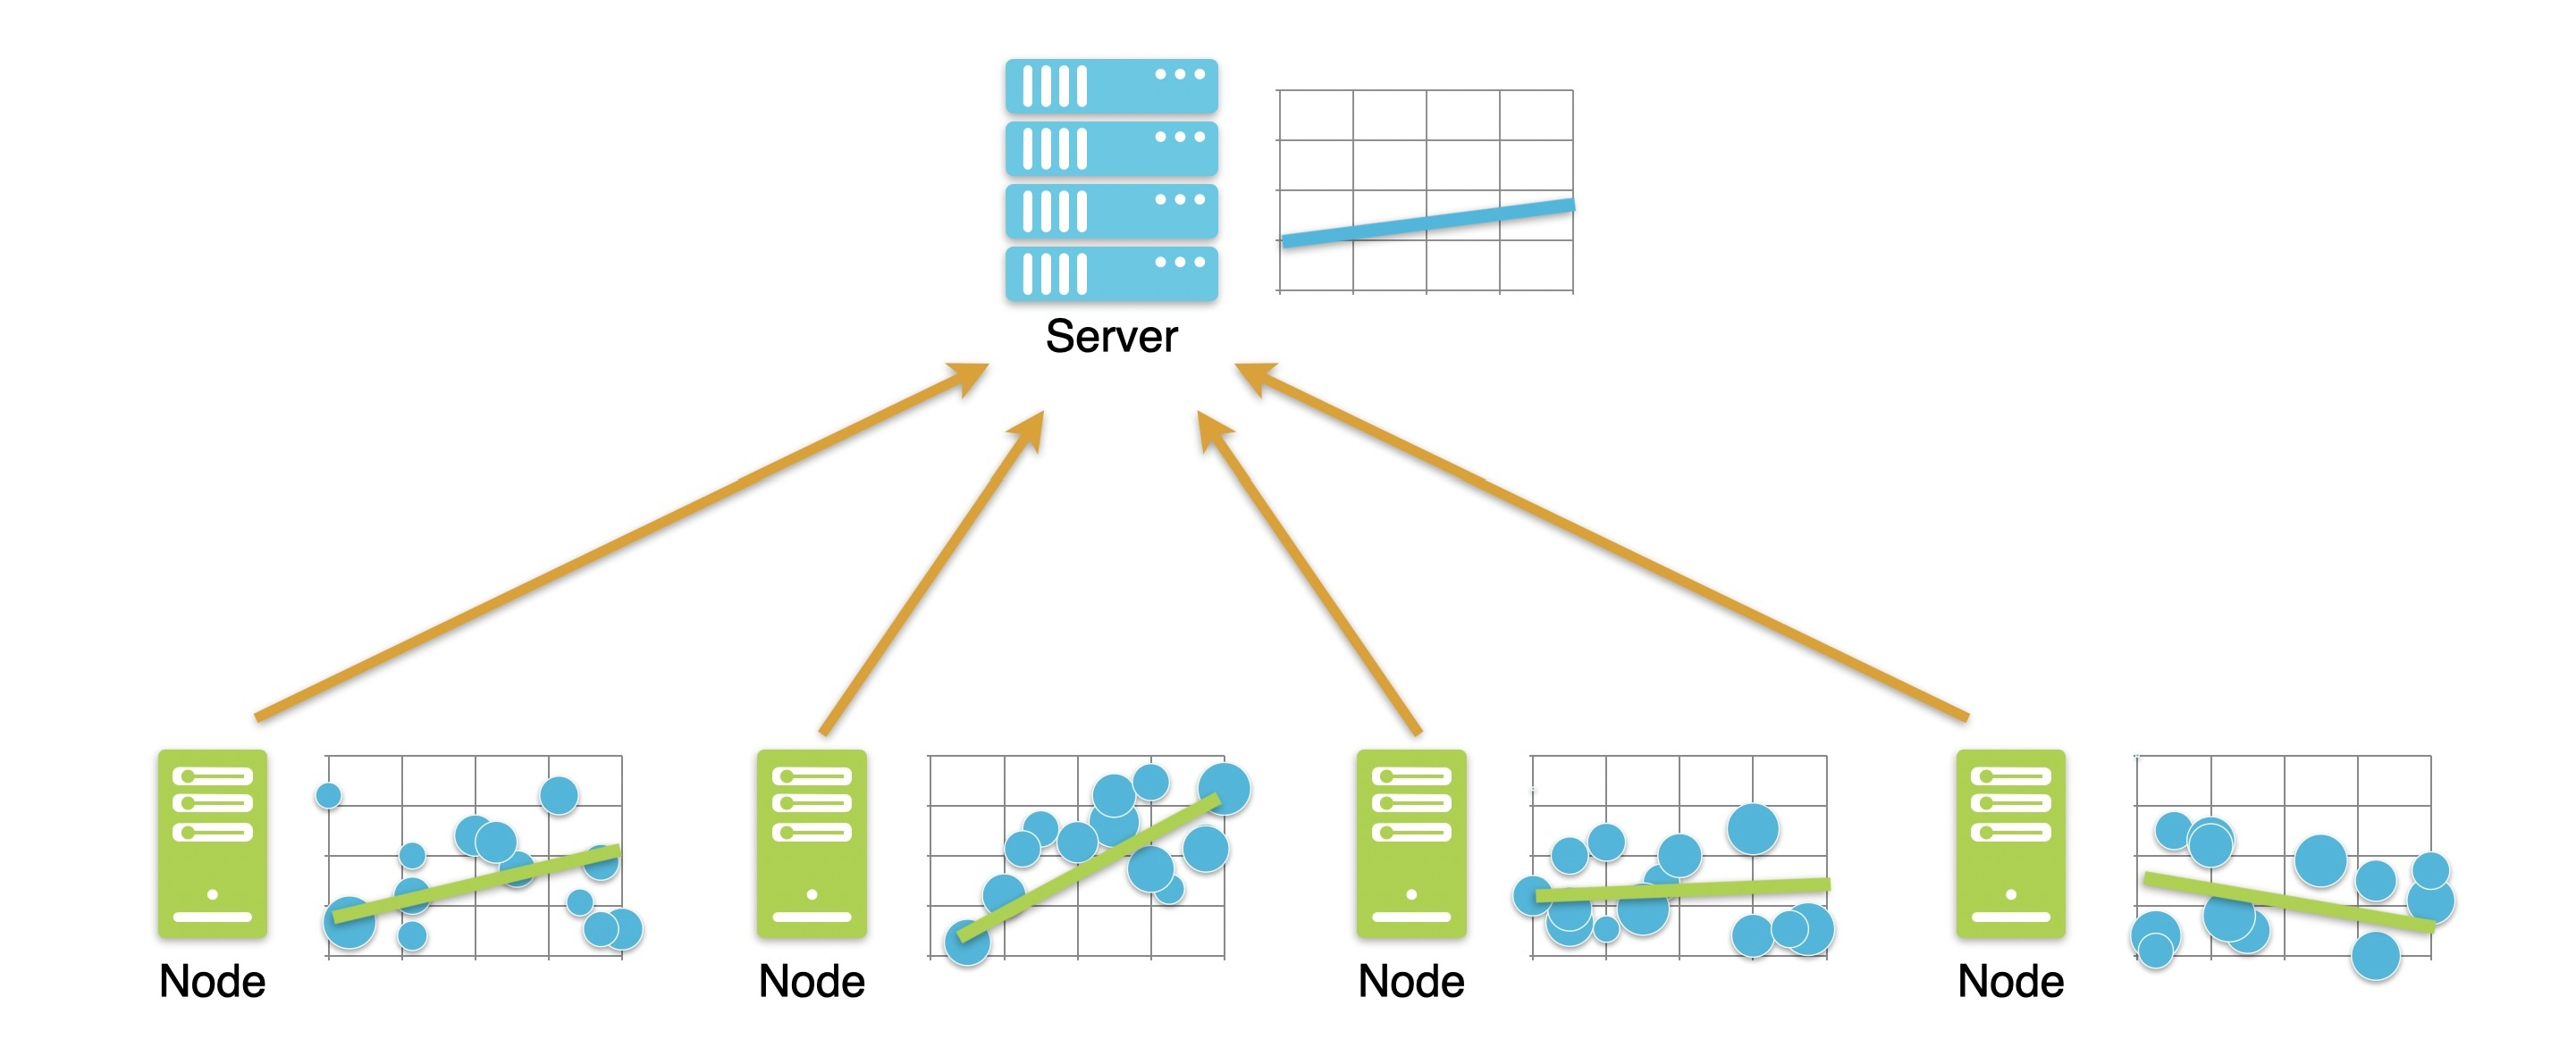
\includegraphics[width=\linewidth]{img/FL-phase2.jpg}
    \vspace*{-.8cm}
    \caption{Models modified by nodes, by integrating local data, are returned to the server}
    \label{fig:fl-phase2}
\end{figure}

Despite its promising potential, \gls{fl} faces several challenges, including power consumption, dropped connections or high-latency due to stragglers, especially in cross-device settings.
Moreover, other issues must be considered, such as adversarial behaviors targeting performance or privacy.
These challenges require robust solutions such as end-to-end encryption and secure aggregation to safeguard data integrity and confidentiality.

%% DIFFERENT APPROACH OF FL
\subsection{Different Approaches of FL}

Two main types of federation coexist, depending on the context and its requirements: \gls{cdfl} and \gls{csfl}.

\paragraph*{Cross-device FL} In \emph{cross-device} settings, the participating devices are typically heterogeneous and widely distributed, encompassing a massive number of parties, such as smartphones, IoT devices and personal computers, potentially ranging from thousands to billions, each device having a small dataset.
Due to the diversity of devices and their varying computational capabilities, cross-device \gls{fl} often encounters challenges related to limited availability, reliability, and communication overhead, but offers scalability and adaptability, making it suitable for scenarios where a large and diverse set of devices is used to train a single model for a third party.

\paragraph*{Cross-silo FL} In contrast, \emph{cross-silo} \gls{fl} operates within organizational boundaries or distinct data silos, where each silo represents a separate entity or institution.
Silos could correspond to different departments within a company, independent organizations, or even geographical regions.
Unlike \gls{cdfl}, which involves heterogeneous devices, \gls{csfl} typically implies organizations with more homogeneous capabilities and more data to train on.
Parties in cross-silo \gls{fl} are more likely to be reliable and consistently available for participation, as they are usually institutional entities with dedicated infrastructure and resources.
Yet, entities involved in \gls{csfl} also tend to have considerably greater discrepancies in terms of objectives and data-distributions, and sometimes even model architectures.
Cross-silo \gls{fl} offers more control over data governance and security, as data sharing occurs within predefined organizational boundaries, facilitating compliance with regulatory requirements and privacy policies.
%\end{itemize}

On the other side, the typical server-orchestrated is challenged in the literature with other forms of architecture aimed at removing this single point of failure, from hierarchical aggregation mechanisms to fully decentralized settings.
Each then introduces its own set of benefits and constraints, although those are beyond the scope of this tutorial.

% \subsection{Wide Acceptance of the Paradigm}

% As evidenced by its exponential growth in research (from a few dozens in the first years to thousands of publications today) and real-world deployments, \gls{fl} stands as a burgeoning field with profound implications for various industries.
% With open-source libraries like PySyft and TensorFlow Federated facilitating its adoption, \gls{fl} fosters interdisciplinary collaboration, bridging machine learning, privacy, and networked systems to shape the future of decentralized intelligence.


\section{Federated Learning for Collaborative Network Security} % Léo
\label{sec:fids}

%% AI in network security
% The increasingly complex and heterogeneous nature of network environments has necessitated the deployment of \gls{ai} and \gls{ml} techniques to properly detect and mitigate security threats.

% In this context, \gls{ai} can intervene at various stages of the network security lifecycle, from threat detection (\eg, \glspl{ids}) to alert correlation and triage (\eg, in \glspl{siem}).
% \Glspl{ai}-enriched \glspl{ids} have emerged as a critical component of modern network security architectures, enabling organizations to timely detect security incidents.
% \Gls{dl} techniques, in particular, have shown promising results in enhancing the performance of \glspl{ids} by allowing for learning more complex patterns and behaviors, and generalizing to zero- or one-day attacks.

\Gls{ai} can intervene at various stages of the network security lifecycle, from threat detection to alert correlation and triage.
%In particular, \glspl{ai}-enriched \glspl{ids} have emerged as a critical component of modern network security architectures, enabling organizations to timely detect security incidents.
\Gls{dl} techniques, in particular, have shown promising results in improving the performance of \glspl{ids} by allowing more complex patterns and behaviors to be learned, and generalizing to zero- or one-day attacks.
%% FL for intrusion detection
Yet, training \gls{dl}-based \glspl{ids} requires large amounts of labeled data to properly learn the underlying patterns of normal and malicious behaviors.
In practice, organizations often face challenges in collecting and sharing such data due to privacy concerns, such as sensitive information leakage or regulatory compliance.
\Gls{fl} offers a compelling solution to this problem by enabling organizations to collaboratively train \gls{ids} models without sharing raw data.

%% CIDS / FIDS
Typical \gls{fl} applications often imply cross-device settings, with the hypothesis of a single actor trying to learn from multiple devices without accessing their data.
The \gls{cids} use case is slightly different, as it usually involves multiple organizations, each owning independent datasets and infrastructures.
We refer to \gls{cids} leveraging \gls{fl} as \gls{fids}, as they are federated across organizations.
%
%% Data heterogeneity
This context raises new challenges, notably the heterogeneity of the data distributions across organizations.
These differences can further vary in terms of monitored traffic (\eg, services, protocols, user behavior), the deployed security solutions, or even the \gls{dl} models used.
The last point is particularly critical, as it prevents the direct aggregation of models as done by \texttt{FedAvg}~\cite{mcmahan_communication-efficient_2017}.

Simplifying the problem, we can consider the case of a shared model architecture, ensuring the applicability of most \gls{fl} strategies.
Yet, the data heterogeneity remains a significant challenge, as model aggregation of highly heterogeneous data is already identified as an open challenge in \gls{fl} literature~\cite{zhu_federated_2021}.

%% Sota
Previous works~\cite{lavaur_evolution_2022} provided a comprehensive overview of the state-of-the-art of \glspl{fids}, identifying clear research directions.
These challenges span over three main axes:

\begin{enumerate}[(i)]
    \item \emph{Transferability, adaptability, and scalability.}
    How to deal with a high number of clients and constrained environments?
    How to learn from heterogeneous data, or heterogeneous clients?
    How to balance generalization and specialization for model aggregation?

    \item \emph{Security, trust, and resilience.}
    How to resist to poisoning and inference attacks against the aggregated models?
%    How to protect sharing and aggregation?
    How to deal with untrusted or malicious participants?
    How to leverage \gls{fl} to react to attacks?

    \item \emph{Local algorithm and aggregation performance.}
    What is the impact of the hyper- and meta-parameters?
    How to model behaviors to better characterize traffic?
    How to improve the raw performance of models?
\end{enumerate}


\section{Security Challenges in Federated Learning} % Léo
\label{sec:threats}

\subsection{Threats against Federated Learning}

%% Threats against FL in IDS context
% - against the model
% - against privacy
The distributed nature of \gls{fids} opens the way to various attack vectors, ranging from poisoning attacks to privacy breaches.
The former aim at altering the global model's behavior, while the latter target the confidentiality of the data used by the participants' in training.
We especially focus on the poisoning attacks, as they are particularly relevant in the context of \gls{fids}~\cite{lavaur_icdcs_demo}.
Indeed, the ability to manipulate the global model is a significant threat, as it can lead to an overall decrease in the security of the protected system.
\citet{rodriguez-barroso_survey_2023} summarizes the different types of poisoning attacks in a fourfold taxonomy:

\begin{enumerate}[(i)]
\item \emph{Attack Moment}: whether the attack is performed during the training or inference phases.

\item \emph{Attackers' Objective}: targeted/backdoor attacks aim at specific samples or classes, modifying the model's behavior when subjected to specific behaviors, while untargeted poisoning alters the global model uniformly.

\item \emph{Poisoned components}: the attack can target the data, the model, or the communication channel.

\item \emph{Frequency}: one-shot attacks or adaptive/iterative ones; in the latter case, different strategies can be adopted, \eg, increasing the percentage of data over time to slowly divert the global model of its original local optimum.
\end{enumerate}


% %% Different threat models
% Depending on the attacker's positioning and knowledge, different threat models can be considered.
% %\begin{enumerate}

%     \paragraph*{Outsider \vs Insider}
%     An outsider has no knowledge of the model or the data used and cannot interact with the system, while an insider has access to the model and its own local data.
%     Further, insiders can impact the model's behavior, and therefore the other participants, while outsiders are limited to listening to the communication channel.
    
%     \paragraph*{Lone \vs Colluding Attackers}
%     Especially in the context of insiders, attackers can act alone or in collusion to maximize their impact.
%     This collusion can be caused by a single entity controlling clients (Sybils) or multiple entities sharing a common interest.
    
%     \paragraph*{Honest-but-curious \vs malicious clients}
%     Honest-but-curious clients follow the protocol but try to learn from the model or the data, while malicious clients actively try to disrupt the system.
% %\end{enumerate}

%% Attack taxonomy


%% Mitigation strategies

\subsection{Mitigation strategies}

Fortunately, the community also proposed numerous mitigation strategies against adversarial attacks targeting \gls{fl} systems and \gls{fids} by extension.
Specifically, multiple works have focused on the development of robust aggregation algorithms and contributions filtering mechanisms, which can mitigate the effect of poisoning attacks.
These strategies can be classified into three main categories:

%\begin{enumerate}
\paragraph*{Server-side evaluation} the server evaluates the received contributions on a purpose-built representative dataset.
This is mostly inapplicable in \gls{niid} settings, as building a representative dataset would imply having access to the clients' data-distribution.
    
\paragraph*{Server-side model comparison} the server compares the received contributions to a reference model, or to each other.
In the former, just as in the previous case, the absence of a single-source-of-truth in \gls{niid} settings makes this approach difficult.
However, by comparing models with each other, the server can detect discrepancies and identify potential malicious contributions.
This is the strategy leveraged by \texttt{FoolsGold} or \texttt{FLAME}, although with different approaches and objectives.

\paragraph*{Client-side evaluation} the clients are tasked to evaluate the contributions of other participants and generate metrics using their local dataset.
This removes the need for a single source of truth, while the metrics act as feedbacks that can be used to feed reputation systems.
%\end{enumerate}

\printbibliography


% \subsection*{Yann Busnel}

% Yann Busnel is Senior Vice-President for Research at the Institut Mines-Télécom (IMT), France.
% With several years of experience within the IMT group, particularly at IMT Atlantique and IMT Nord Europe, he is responsible for developing and implementing the institution's scientific strategy.
% His work involves fostering inter-affiliate collaborations, overseeing doctoral programs, managing the PhD diploma of IMT, and coordinating the activities of its 11 scientific communities.
% He has over 15 years of experience in research and higher education.
% Between June 2023 and September 2024, he served as Director of Research and Innovation at IMT Nord Europe.
% Before that, he has held various academic positions and responsibilities in France and abroad: Full Professor at IMT Atlantique, Associate Professor at ENSAI in Rennes, Assistant Professor at the University of Nantes, and Researcher at Sapienza University of Rome.

% His research topics are mainly related to Models for large-scale distributed systems and networks, with application in Data stream analysis, Cybersecurity, Massive health data and Artificial Intelligence. Recently, his areas of application range from (1) cybersecurity and dependability to (2) the analysis of medical data, in the context of pharmacovigilance or genomic sequence analysis, and (3) the self-organized coordination of fleets of drones. He has published over 100 articles in peer-reviewed journals and conferences. He has also coordinated several national and international collaborative research projects, and is currently a member of the steering committee of the French national research group on networks and distributed systems (GDR RSD).

\begin{IEEEbiography}%
    [{
\includegraphics[width=1in,height=1.25in,clip,keepaspectratio]{img/yann.jpg}}]%
    {Yann Busnel} is Senior Vice-President for Research at the Institut Mines-Télécom (IMT), France. With several years of experience within the IMT group, particularly at IMT Atlantique and IMT Nord Europe, he is responsible for developing and implementing the institution's scientific strategy. His work involves fostering inter-affiliate collaborations, overseeing doctoral programs, managing the PhD diploma of IMT, and coordinating the activities of its 11 scientific communities. He has over 15 years of experience in research and higher education. Between June 2023 and September 2024, he served as Director of Research and Innovation at IMT Nord Europe. Before that, he has held various academic positions and responsibilities in France and abroad: Full Professor at IMT Atlantique, Associate Professor at ENSAI in Rennes, Assistant Professor at the University of Nantes, and Researcher at Sapienza University of Rome.

    His research topics are mainly related to Models for large-scale distributed systems and networks, with application in Data stream analysis, Cybersecurity, Massive health data and Artificial Intelligence. Recently, his areas of application range from (1) cybersecurity and dependability, to (2) the analysis of medical data, in the context of pharmacovigilance or genomic sequence analysis, and (3) the self-organized coordination of drone fleets. He has published over 100 articles in peer-reviewed journals and conferences. He has also coordinated several national and international collaborative research projects and is currently a member of the steering committee of the French national research group on networks and distributed systems (GDR RSD).
\end{IEEEbiography}

\begin{IEEEbiography}%
    [{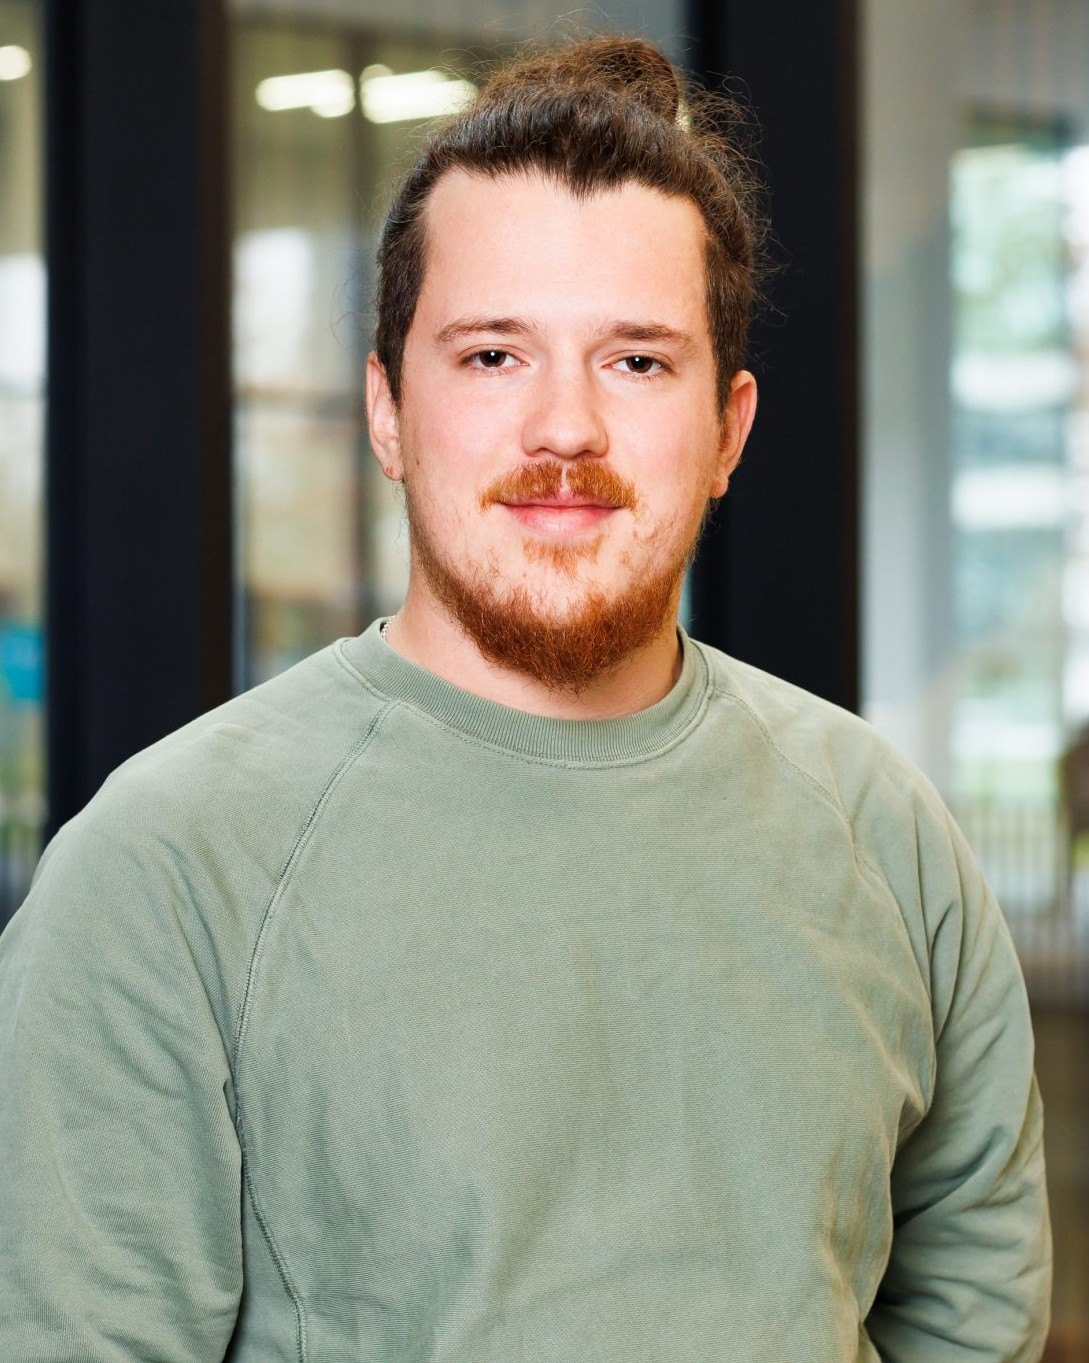
\includegraphics[width=1in,height=1.25in,clip,keepaspectratio]{img/leo.jpg}}]%
    {Léo Lavaur} is Researcher at the Interdisciplinary Centre for Security, Reliability and Trust (SnT), University of Luxembourg. He received his Ph.D. in cybersecurity from IMT Atlantique, France, in 2024, where he focused on applying Federated Learning to Collaborative Intrusion Detection. During his Ph.D., he collaborated closely with the Chair on Cybersecurity in Critical Networked Infrastructures (Cyber CNI) and its industrial partners, who partially funded his research. He holds an Engineering degree in Information Security from ENSIBS, Vannes, France. During his studies, he also worked part-time at Orange Cyberdefense.

    His research explores various aspects of distributed system security, with a particular emphasis on collaborative knowledge sharing through machine learning. His research interests range from federated and decentralized learning to network security and intrusion detection, including the application reproducibility and the evaluation of distributed intrusion detection approaches. He has published several papers on the application of Federated Learning to network security, focusing on the challenges of data heterogeneity and dealing with adversarial behaviors. His current research focuses on modeling causal dependencies in distributed microservice and GenAI architectures.
\end{IEEEbiography}
% \subsection*{Léo Lavaur}

% Léo Lavaur is a Researcher at the Interdisciplinary Centre for Security, Reliability and Trust (SnT), University of Luxembourg.
% He received his Ph.D. in cybersecurity from IMT Atlantique, France, in 2024, where he focused on applying Federated Learning to Collaborative Intrusion Detection.
% During his Ph.D., he collaborated closely with the Chair on Cybersecurity in Critical Networked Infrastructures (Cyber CNI) and its industrial partners, who partially funded his research.
% He holds an Engineering degree in Information Security from ENSIBS, Vannes, France. During his studies, he also worked part-time at Orange Cyberdefense.

% His research explores various aspects of distributed system security, with a particular emphasis on collaborative knowledge sharing through machine learning.
% His research interests range from federated and decentralized learning to network security and intrusion detection, including the application reproducibility and the evaluation of distributed intrusion detection approaches.
% He has published several papers on the application of Federated Learning to network security, focusing on the challenges of data heterogeneity and dealing with adversarial behaviors.
% His current research focuses on modeling causal dependencies in distributed microservice and GenAI architectures.


% % OLD
% His contributions range from applying Federated Learning to network security to ensuring the security of FL architectures themselves.
% He also has ongoing research activities on dataset generation, model evaluation, and data-quality challenges in FL, as well as communication-efficient decentralized learning.
% He currently focuses on modeling causal dependencies in distributed microservice and GenAI architectures.

\vfill


\end{document}